\section{Gráficos}
Todos os gráficos foram gerados usando a ferramenta de geração de gráfico do 
\citeonline{LOcalc}.
\subsection{Média do Tempo Total de Execução Dos Testes}
\subsubsection{Faixa 1}

blabla
\begin{figure}[htb]
	\centering
	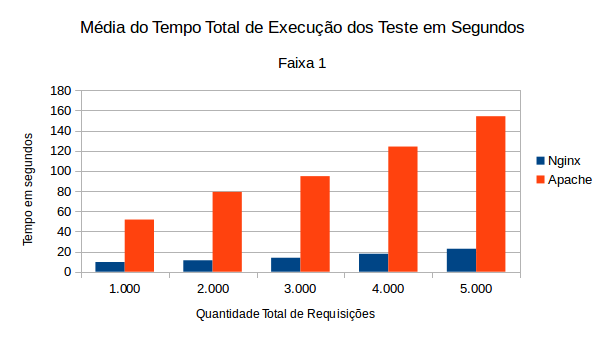
\includegraphics[width=0.6\linewidth]{graficos/grafico1-f1} 
	\caption{Média do Tempo Total de Execução dos Testes - Faixa 1}
	\label{fig:grafico1-f1}
\end{figure}

blabla

\subsubsection{Faixa 2}
blabla

\begin{figure}[htb]
	\centering
	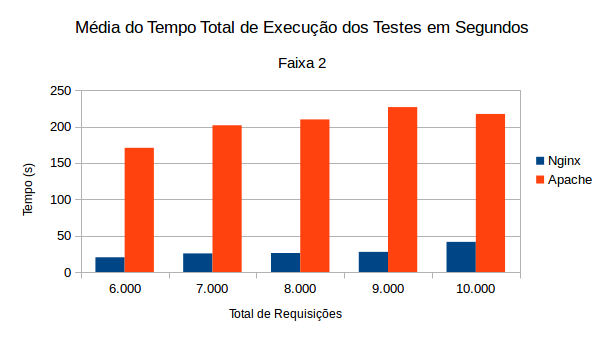
\includegraphics[width=0.6\linewidth]{graficos/grafico1-f2} 
	\caption{Média do Tempo Total de Execução dos Testes - Faixa 2}
	\label{fig:grafico1-f2}
\end{figure}
blabla

\subsubsection{Faixa 3}
blabla

\begin{figure}[htb]
	\centering
	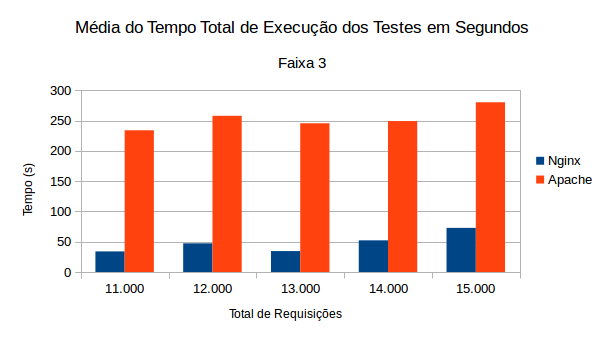
\includegraphics[width=0.6\linewidth]{graficos/grafico1-f3} 
	\caption{Média do Tempo Total de Execução dos Testes - Faixa 3}
	\label{fig:grafico1-f3}
\end{figure}
blabla


\subsection{Média da Quantidade Total de Dados Transmitidos}
\subsubsection{Faixa 1}

blabla
\begin{figure}[htb]
	\centering
	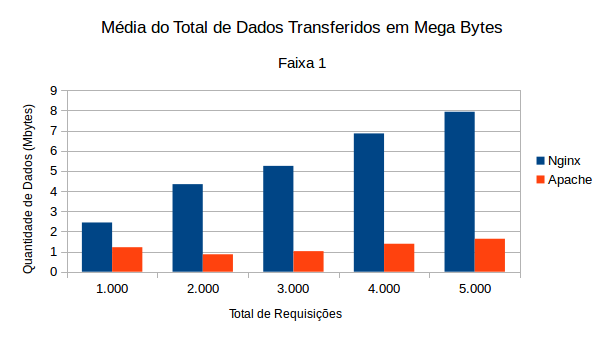
\includegraphics[width=0.6\linewidth]{graficos/grafico2-f1} 
	\caption{Média do Total de Dados Transferidos - Faixa 1}
	\label{fig:grafico2-f1}
\end{figure}

blabla

\subsubsection{Faixa 2}
blabla

\begin{figure}[htb]
	\centering
	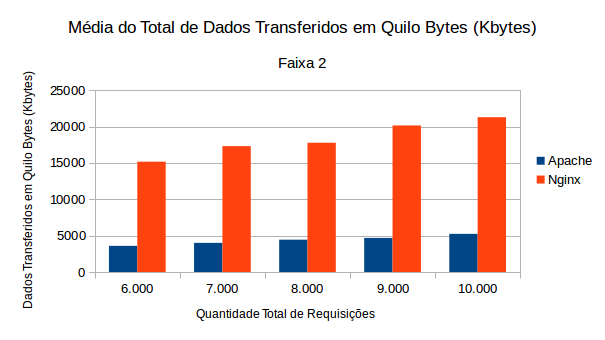
\includegraphics[width=0.6\linewidth]{graficos/grafico2-f2} 
	\caption{Média do Total de Dados Transferidos - Faixa 2}
	\label{fig:grafico2-f2}
\end{figure}
blabla

\subsubsection{Faixa 3}
blabla

\begin{figure}[htb]
	\centering
	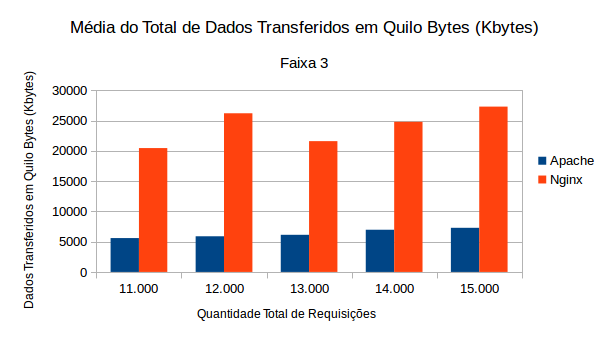
\includegraphics[width=0.6\linewidth]{graficos/grafico2-f3} 
	\caption{Média do Total de Dados Transferidos - Faixa 3}
	\label{fig:grafico2-f3}
\end{figure}
blabla

\subsection{Média da Quantidade de Texto HTML Transmitido}
\subsubsection{Faixa 1}

blabla
\begin{figure}[htb]
	\centering
	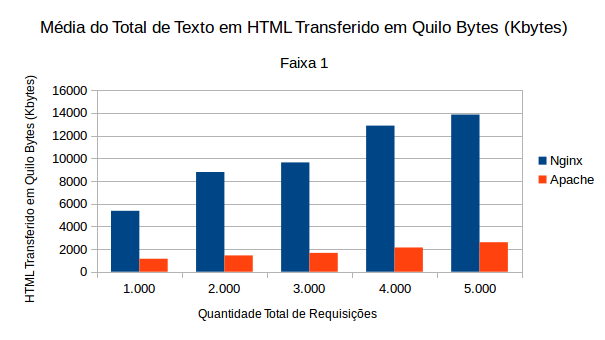
\includegraphics[width=0.6\linewidth]{graficos/grafico3-f1} 
	\caption{Média do Total de Texto em HTML Transferido - Faixa 1}
	\label{fig:grafico3-f1}
\end{figure}

blabla

\subsubsection{Faixa 2}
blabla

\begin{figure}[htb]
	\centering
	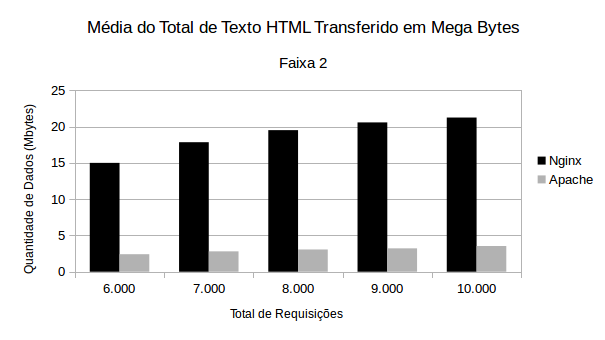
\includegraphics[width=0.6\linewidth]{graficos/grafico3-f2} 
	\caption{Média do Total de Texto em HTML Transferido - Faixa 2}
	\label{fig:grafico3-f2}
\end{figure}
blabla

\subsubsection{Faixa 3}
blabla

\begin{figure}[htb]
	\centering
	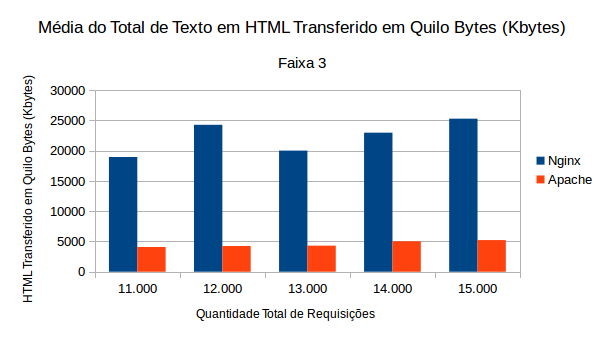
\includegraphics[width=0.6\linewidth]{graficos/grafico3-f3} 
	\caption{Média do Total de Texto em HTML Transferido - Faixa 3}
	\label{fig:grafico3-f3}
\end{figure}
blabla